-This chapter will describe how the system will be designed, how the Field of application can be modelled, what functionalities can be planned-

\section{Einsatzgebiet}
Um präzise beschreiben zu können was das System tun können muss, ist es notwendig vorher konkret die vorliegende Situation oder das existierende Problem zu definieren. Solche eine Definition sollte eine Beschreibung der Umgebung beinhalten in der das System eingesetzt werden soll. Nimmt man eine Modellierungssprache zur Hilfe, um die Umgebung zu beschrieben, ist es später einfacher daraus Rückschlüsse auf mögliche Probleme zu ziehen. Für ein solches Modell müssen die Fragen beantwortet werden, in welche Objekte sich die Umgebung aufgliedert, wie diese interagieren und welche Funktionalitäten diese dafür verwenden.Aber auch die teilhabenden Akteure und ihre konkreten Anforderungen an das System müssen modelliert werden. Mit Hilfe von exemplarischen Anwendungsfällen werde ich beschreiben was der tatsächliche Bedarf des Nutzers ist, und wie dieser gedeckt werden kann.

Bevor ich mit dem technischen Ausformulieren der Modellierung beginne, möchte ich kurz in die Thematik einleiten: Das System welches ich mit dieser Arbeit konzeptioniere soll Feldingenieuren helfen im Feld mit den Messungen und Daten verschiedener Sensoren zu arbeiten. Als konkretes Beispiel werde ich den Einsatz des Systems bei der Bauwerksüberwachung mithilfe eines Sensornetzwerkes beschreiben.

Die Überwachung von Bauwerken mittels eines Netzwerkes aus verschiedenen Sensoren hilft ihre Sicherheit ohne den Einsatz großer Bautechnischer Überprüfungen einschätzen zu können. Damit ist es möglich Bauwerke auch weit über ihre geplante Lebensdauer hinweg zu erhalten. Ohne den Einsatz solcher Sensor Netzwerke können die zuständigen Gutachter bei Ablauf der geplanten Lebensdauer nicht darauf vertrauen, dass das Gebäude auch weiterhin den kontinuierlichen Belastungen gewachsen ist, und somit werden entweder umfangreiche Sanierungen Nötig, oder Gebäude werde geschlossen. Die Überwachung basiert auf der Messung von Veränderungen von verschiedenen Parametern wie zum Beispiel der Position , der Temperatur oder Feuchtigkeit von Bauteile oder der Abweichungen von charakteristischen Bewegungsmustern von Bauteilen, gemessen durch Beschleunigungssensoren. Die Parameter werden sowohl punktuell  verteilt über das gesamt Bauwerk, als auch gesamtheitlich die Struktur des Bauwerkes miteinbeziehend erhoben, siehe auch \citep{worden_overview_2004} \citep{farrar_introduction_2007} \citep{boller_structural_2004}. Für die Messungen werden zum einen automatisch kontinuierlich messende Systeme eingesetzt, und zum anderen seltenere manuelle Messungen, deren Ergebnisse manuelle in das System eingegeben werden. 

Für das bessere Verständnis möchte ich hier ein Beispielfall beschreiben: Ein Brücke erreicht ihre letzten Jahre der Betriebserlaubnis. Danach müssen entweder die Verkehrssicherheit erneut umfangreich geprüft, und zahlreiche Verschleißteile, deren Zustand schlecht zu beurteilen ist, ersetzt werden, oder die Verkehrssicherheit muss auf andere Art überprüft werden. Zahlreiche Sensoren werden an den einzelnen wichtigen Gebäudeteilen eingerichtet, und überwachen nun automatisch über einen bestimmten Zeitraum deren Verhalten und Veränderungen. In periodischen Abständen werden automatisch Diagnosen erstellt, basierend auf der Analyse der Messwerte, der Überprüfung des Materialverschleißes und einiger anderer Einflussgrößen. Eine detailliertere Beschreibung der verwendeten Messungen, Zeitskalen und Analysemethoden werden in den nachfolgenden Kapiteln beschrieben.

In der Einleitung der Arbeit möchte ich mich am Verlauf der Erstellung eines Pflichtenheftes für die Softwareentwicklung orientieren , da so am besten modelliert werden kann wie der Bedarf des Nutzers gedeckt werden kann, siehe auch \citep{gregor_engels_vorlesung_2006}. Beginnen werde ich mit einer textuellen Beschreibung der Situation. Danach folgt eine Modellierung der Prozesse und der Akteure mit ihren jeweiligen Anwendungsfällen. Zum Abschluss werde ich dann die daraus abgeleiteten notwendigen Funktionalitäten des System beschreiben.


\subsection{Modell des Problembereichs}
Die Abbildung \ref{fig:model_domain} zeigt ein UML Diagramm (Unified Modeling Language) das die im folgenden beschrieben verschiedenen Objekte des Systems beinhaltet. Das Modell beschreibt die Beziehungen der einzelnen Objekte untereinander und modelliert keine Aktivitäten oder Funktionen.

Die Umgebung in der das System eingesetzt werden wird besteht aus fünf verschiedenen Arten von Objekten und deren Beziehungen untereinander. Zentrales Objekt ist der Daten Server, der als Knoten für die Kommunikation zwischen den einzelnen Kompartimente dient. Diese sind hauptsächlich die Sensoren selbst, die jedoch ohne einen Server, der als Steuerungseinheit für jeden Sensor dient, nicht selbständig messen können. Der Server kontrolliert die Sensoren indem er sie aktiviert und deaktiviert. Nichtsdestotrotz können Sensoren in einem separiertem eigenem Netzwerk organisiert sein, das dann wiederum als einzelner Sensor behandelt wird. Die Sensoren senden ihre gemessenen Daten entweder aktiv an den Server beziehungsweise über den Server an die dem Server angeschlossene Datenbank, oder der Server ruft die Daten aktiv ab, und speichert diese dann in der Datenbank.

\begin{figure}[H]
	\centering
 	 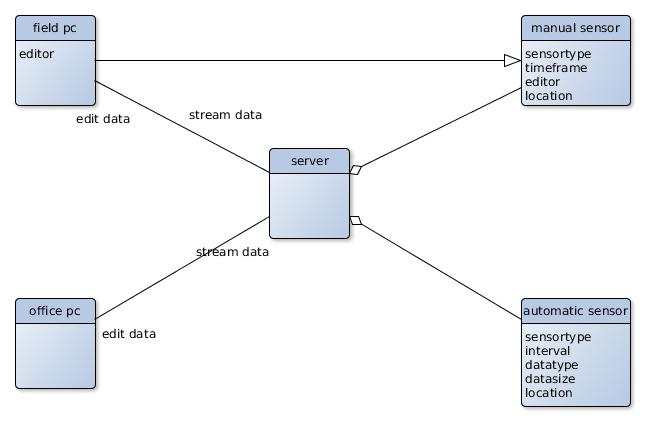
\includegraphics[scale=0.6]{graphics/model_of_issue.jpg} 
	\caption{Modell des Problembereiches mit relevanten Objekten, F. H. Euteneuer 2013}
	 \label{fig:model_domain}
\end{figure}

Die Datenbank die and den Server angeschlossen ist speichert sowohl Metadaten zu den Sensoren, als auch die gemessenen Werte. Unter Metadaten sind alle Informationen zu verstehen, die die Sensoren eindeutig beschreiben, und die für weitere Analysen der Messerwerte erforderlich sind (siehe auch im Glossar "Metadaten". Beispielsweise sind das die Positionen der Sensoren, die Messintervalle, die Sensortypen oder die übermittelten Datentypen.

Als Klient des Services kann im Prinzip jede Art von mobilen Systemen eingesetzt werden. Angeschlossen an die Datenbank dienen diese dann als bildgebender Teil des Systems. Da die Verknüpfung mit einem Server meist über das Protokoll TCP/IP geschieht, müssen mobile Geräte über eine Internetverbindung verfügen. Die Verwendung dieser Geräte bleibt dadurch begrenzt auf Gebiete innerhalb der Handynetz-Abdeckung. Für manuelle Messungen dient der mobile Klient zusätzlich als Eingabegerät für die Messwerte, sofern dies nicht über das Gerät selber erfolgen kann. Dadurch wird der mobile Klient in dem Modell sowohl als bildgebender Teil des Systems, als auch als Sensor behandelt, und ererbt damit die Eigenschaften des Sensor Objekts.

Das System will einen ganzheitlichen Ansatz verfolgen, und beinhaltet somit auch einen Teil der für die umfangreicheren Analysen zuständig ist, sowie durch eine Datenexportfunktion als Schnittstelle zu weiteren Algorithmen und System dient. Dieser Teil des System wird in dem Modell durch den "Desktop-Computer" repräsentiert. Die eigentliche Einrichtung und Planung des Systems wird erwartungsgemäß von diesem, dem bequemeren Arbeitsplatz (verglichen mit dem mobilen Klienten), durchgeführt werden. Zusätzlich zu den Eigenschaften des Feldcomputers sind somit erweiterte Verwaltungs- und Analysefunktionen als Eigenschaften dieses Objektes definiert.


\subsection{Geschäftsprozesse}
Wichtigste Entscheidungshilfe für die Nutzung solch eines Systems wird die Eigenschaft des Systems, eine entscheidungsunterstützende Funktion zu erfüllen, sein. Das System ist fokussiert auf die wichtigen Werkzeuge die die Arbeit des Feldingenieurs vereinfachen sollen, und lässt unwichtige oder komplizierte Werkzeuge komplett weg. Außerdem werden die Informationen die im Feld auf dem mobilen Klienten angezeigt werden derart reduziert, dass lediglich aussagekräftige Werte, die damit Entscheidungen unterstützen können, angezeigt werden. In dem vorherigem Kapitel habe ich den Problembereich beschrieben, nun möchte ich die verschiedenen Prozesse skizzieren die ein Nutzer durchführen könnte.

\begin{figure}[H]
	\centering
 	 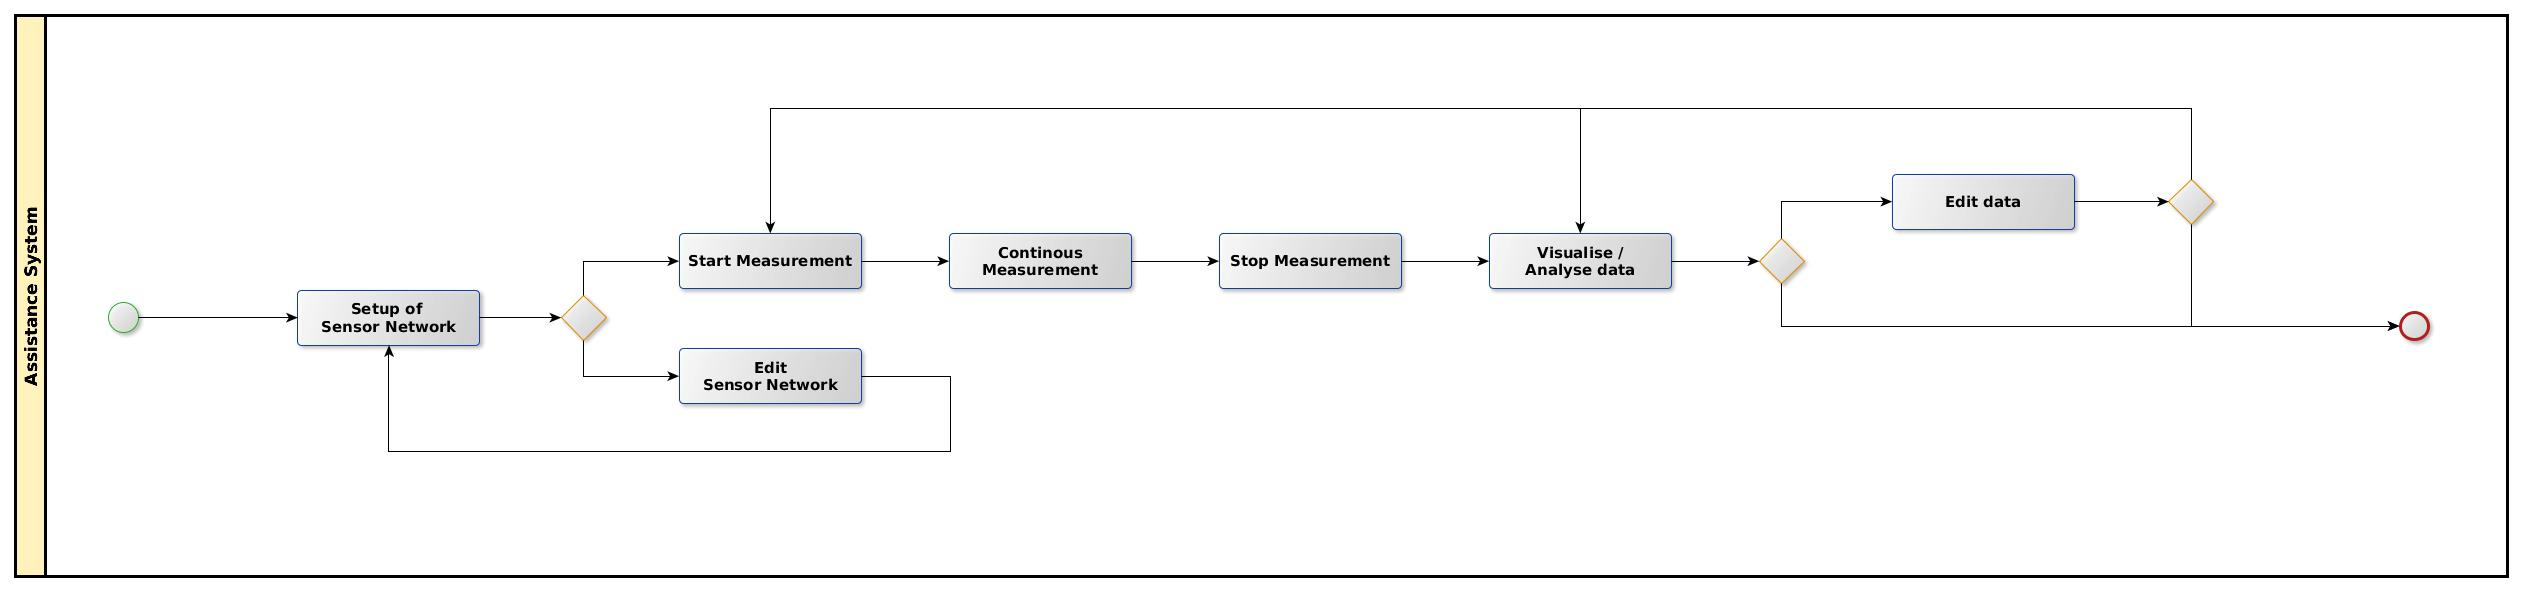
\includegraphics[scale=0.2]{graphics/bpmn_business-processes.jpg} 
	\caption{BPMN (Business Process Model and Notation) Modell relevanter Aktionen welche in dem System durchgeführt werden, F. H. Euteneuer 2013}
	 \label{fig:model_business-processes}
\end{figure}

Ich habe drei verschiedene Hauptaktionen identifiziert, die ein Nutzer durchführen könnte: Das manuelle Messen von Werten, das manuelle Editieren bereits gemessener Werte, und das automatische kontinuierliche Messen. Die Abbildung \ref{fig:model_business-processes} veranschaulicht mittels eines UML Activity Diagrams (UML Aktivitäten Diagramm) die einzelnen Abläufe dieser Aktionen.

Die manuelle Messung beginnt mir der normalen Messung der Werte. Im zweiten Schritt erfolgt die Eingabe der Werte in das System. Die Werte werden automatisch auf ihre Validität hin überprüft, und erste einfache statistische Analysen werden erstellt. Diese erste Statistik ist erforderlich um Informationen über die Qualität der Messung zu erhalten, und dem System die Möglichkeit zu bieten fehlerhafte Messungen zu bemängeln und Neumessungen vorzuschlagen.

Der Nutzer wird die Möglichkeit haben vergangene Messungen manuell zu bearbeiten. Dazu muss ein Datensatz (Üblicherweise ein Messwert) ausgewählt werden, und der Nutzer kann dann entscheiden ob die betreffende Messung wiederholt werden soll, oder die Werte manuell geändert werden sollen. Bei einer Wiederholung der Messung wird die Prozesskette der manuellen Messung durchlaufen.


The automatic measurements are the most important one for the described SHM. The will be the backbone of the system, nevertheless they are using similar functionalities. The user will initially be able to set the sensor network up. Which means to enter metadata about the used sensors like position, reference system, type of sensor, measurement interval, etc. A more detailed description of what is needed for such a setup will follow in the methodical part. After the setup, the user is able to start the measurements with the defined parameter, or the edit the settings.

As a conclusion of this chapter, I would like to point out that this list is only representing functionalities of a basic system, and should not be understood as being complete.


\section{Functionalities}
This chapter will describe what the system should provide to solve the problem and/or make the existing situation better: Which functionalities should be part of the system. To get closer to a possible solution, the different stakeholders and their use cases in the domain of structural health monitoring must be defined and described.

\begin{figure}[H]
	\centering
 	 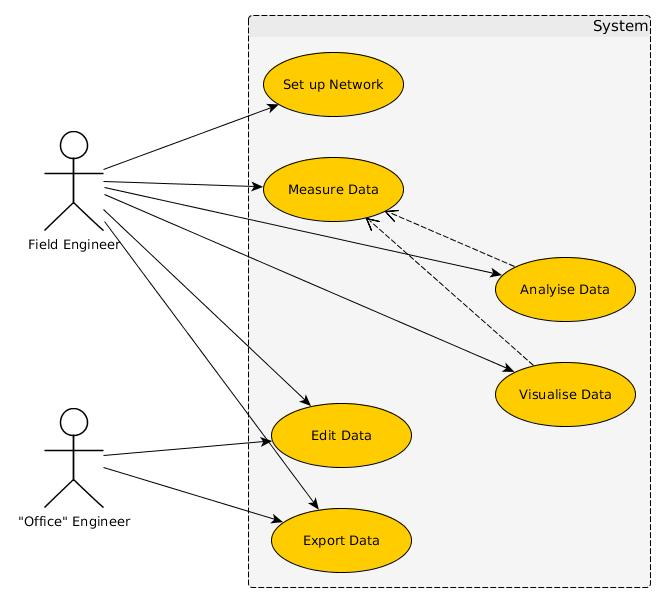
\includegraphics[scale=0.6]{graphics/uml_functionalities.jpg} 
	\caption{UML Use Case Diagram of the described System describing two different users and their use cases. By F. H. Euteneuer 2013}
	 \label{fig:model_functionalities}
\end{figure}

\subsection{Usergroups}
As a main source for information and parameter for the concept of a software, the usergroups are of large importance. I will analyse the involved usergroups and their needs respective expectations to get those information. As the figure \ref{fig:model_functionalities} is already representing, I have identified two main usergroups which might be involved in the processes.

\subsubsection{Field-engineer}
The group of field-engineers can described as the executive persons which are dealing with the direct measurements, observations and setup of an automatic measurement network. This group can be categorised by its technically limits, which are:
\begin{itemize}
\item the small screen-size of the mobile computers (quality of visualisation is limited)
\item the lack of input facilities (e.g. only digital keyboard on a handheld computer)
\item high weight of not handheld instruments (e.g. a conventional laptops too heavy for using while walking/standing)
\end{itemize}
But nevertheless, this usergroup has the most challenging requirements on the system when speaking about visualisation options or analysis computation in advance. It is the central target usergroup for this system, therefore it should fit mostly to its requirements.


\subsubsection{Office-engineer}
Usually the field-engineer and the office-engineer are combined in one person. One part of an observation project is dealing with the field-work, the setup, measurements and maintenance. And the other part is the precise analysis of the data, the post processing and its interpretation. Due to a high quality equipment in the offices, this part is mostly better solvable for a software. Here does not the system has to be restricted by the environment, but the system is making its demands on the technical environment.


\subsection{Use Cases}
The Figure \ref{fig:model_functionalities} is showing the different basic use cases of the described two usergroups. Use cases shown in this figure are representing activities of the user which have to be complete with it own defined target. I want now describe the use cases in detail with further parameter. This is important for the further proceeding of the system conception, because use cases are defining the users interests of a system.

The following part will describe the selected use cases in detail. All the use cases will be described with tables for the textual description which are containing information about the use case goal, the postcondition and further more. For the description of the the chronological task flow of the use cases also a activity diagram will depict each use case.

Important to know is, that the diagrams are not representing all possible activity flows which are available. They are representing one possible option which could solve the problem and will be implemented in the prototype.

The use cases are divided into three different groups. There are use cases dealing with central data management functionalities, others are describing main measurement functionalities and the last are describing the data analysis functionalities.


\subsubsection{Management}
There are several use cases with central management functionalities of the system. Management stands for both, data management and system management.  

First use case within the system is the setting up of the network. It can be understood as the initial task and therefore a kind of a precondition for all other use cases.The table \ref{table:use case description of "Set up network"} is describing central features of this use case. 

The export of the data is another major task within the management field. It could be denoted as the final task interacting with the system. The second table \ref{table:use case description of "Export data"} is showing detailed information about the "Export data" use case.

\begin{table}[H]
\centering
\begin{tabular}{l | p{11cm}}
Name & Set up network\\ \hline 
Usergroup & Field engineer\\ \hline 
Goal & Input all metadata about connected sensors and initialise network\\ \hline 
Precondition & Network physically existing and able to correspond with system\\ \hline 
Postcondition & working network with all sensors\\ 
\end{tabular}
\caption{Use Cases tabular description of characteristics} 
\label{table:use case description of "Set up network"}
\end{table}

\begin{table}[H]
\centering
\begin{tabular}{l | p{11cm}}
Name & Export data\\ \hline 
Usergroup & Office Engineer\\ \hline 
Goal & Specify data by parameter and specify output format\\ \hline 
Precondition & Specified data and output format\\ \hline 
Postcondition & complete dataset in specific format offline\\ 
\end{tabular}
\caption{Use Cases tabular description of characteristics} 
\label{table:use case description of "Export data"}
\end{table}

Figure \ref{fig:bpmn_use-case_management} is showing the systems management use cases in a two line activity diagram. The both activity flows do not have any interaction in between, but chronologically must the setup use case performed before the export use case.

The activity flow of the setup use case is showing two main tasks: The database-setup and the input of the sensor-parameter. Those are the central parts and their success or failure is leading to an overall success or failure. An edit of an existing network is leading to a restart of the full procedure. This could be interpreted as an assistant which is leading through the different configurations and is taking care of possible errors.

The export use case is much easier, it is simply the normal flow which is equal to most of the download assistants which can be found online. The only important information about that is the determination of the export datasets time-frame.

\begin{figure}[H]
	\centering
 	 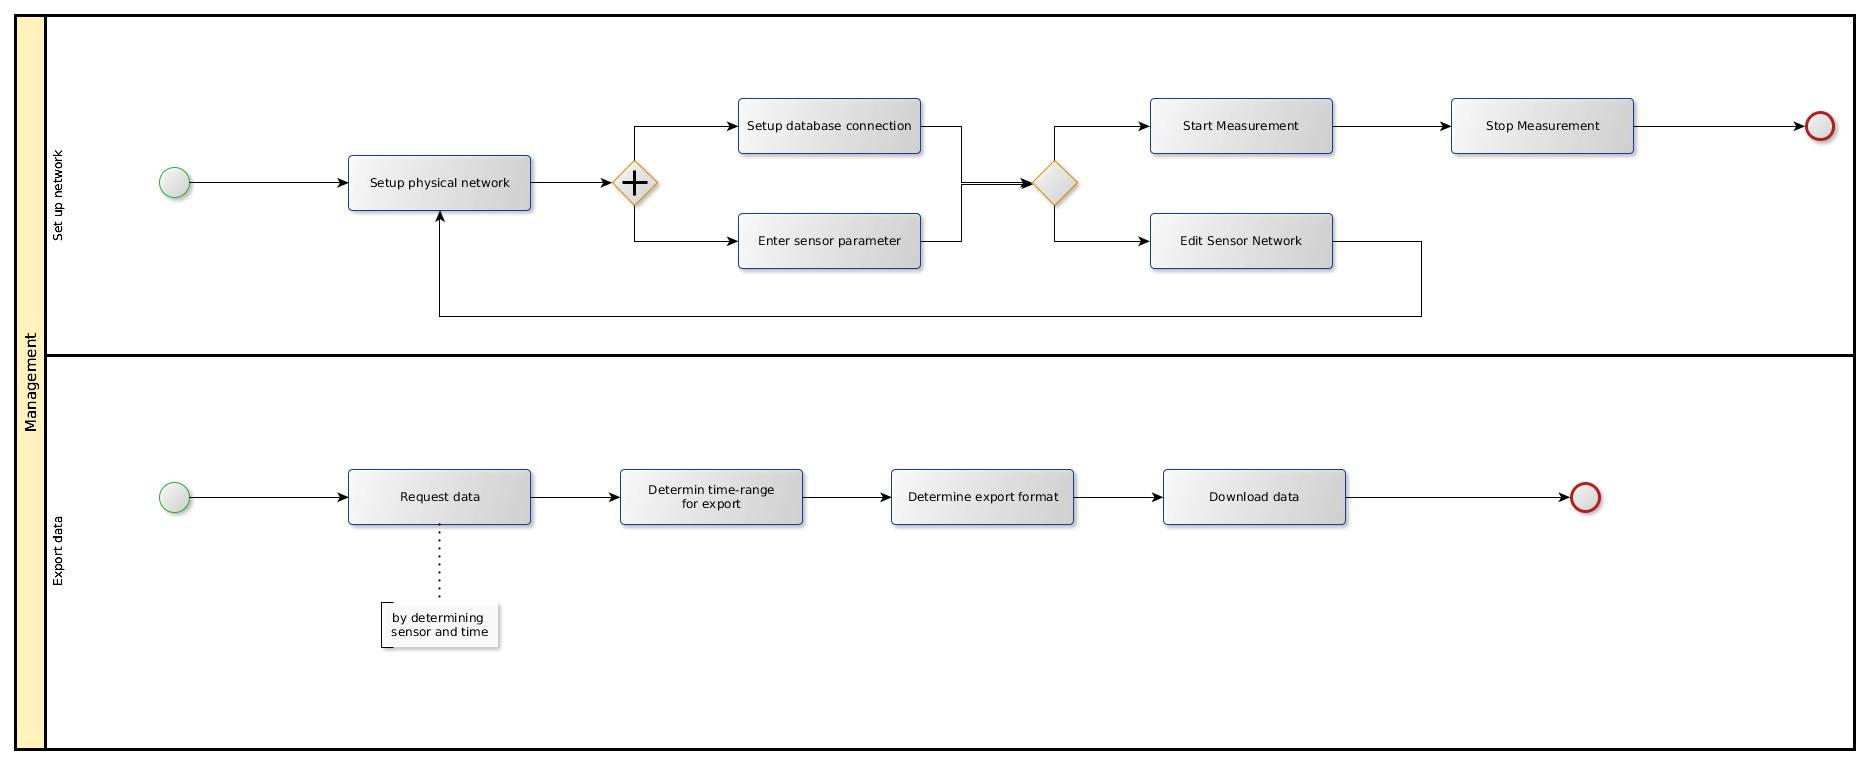
\includegraphics[scale=0.24]{graphics/bpmn_use-cases_management.jpg} 
	\caption{BPMN (Business Process Model and Notation) Model of the use cases describing central management proceedings. By F. H. Euteneuer 2013}
	 \label{fig:bpmn_use-case_management}
\end{figure}


\subsubsection{Measuring}

The measurement part might be the most important one within the system. This part is the only one which is describing a manual manipulation of the data in the database.

There are two identified use cases: The first is dealing with the initial data input which is the measurement see table \ref{table:use case description of "Measure data"}. In contrast to the automatic measurements, this is describing a discrete manual measurement, and the input of the data by hand.

And the second one is editing already existing data in the database see table \ref{table:use case description of "Edit data"}. This is a merely a standard operation for database related systems. Nevertheless, this task is related to the measurement task, in case of re-measuring data or validation of data.

\begin{table}[H]
\centering
\begin{tabular}{l | p{11cm}}
Name & Measure data\\ \hline 
Usergroup & Field engineer\\ \hline 
Goal & Input all data by hand  getting from standalone measurement device\\ \hline 
Precondition & Running system and access to database\\ \hline 
Postcondition & valid data in the database with full set of metadata\\ 
\end{tabular}
\caption{Use Cases tabular description of characteristics} 
\label{table:use case description of "Measure data"}
\end{table}

\begin{table}[H]
\centering
\begin{tabular}{l | p{11cm}}
Name & Edit data\\ \hline 
Usergroup & Office Engineer\\ \hline 
Goal & Specify data by parameter and input new values by hand or measurement\\ \hline 
Precondition & Running system and access to database\\ \hline 
Postcondition & changed data in the database with full set of metadata\\ 
\end{tabular}
\caption{Use Cases tabular description of characteristics} 
\label{table:use case description of "Edit data"}
\end{table}

When performing a manual measurement, most of the task described in the first line of the figure \ref{fig:bpmn_use-case_measuring} will be mandatory tasks. In the end the system will perform a quick analysis of the inserted data in order to validate the measurement. After this step the system will either point out possible errors, or it will approve the measurements, and write them into the database. The second line, the editing flow, is offering two options, one is a manual insert of new data, another would lead to a re-entering of the manual measurement flow, in order to overwrite the selected datasets with new measurements.

\begin{figure}[H]
	\centering
 	 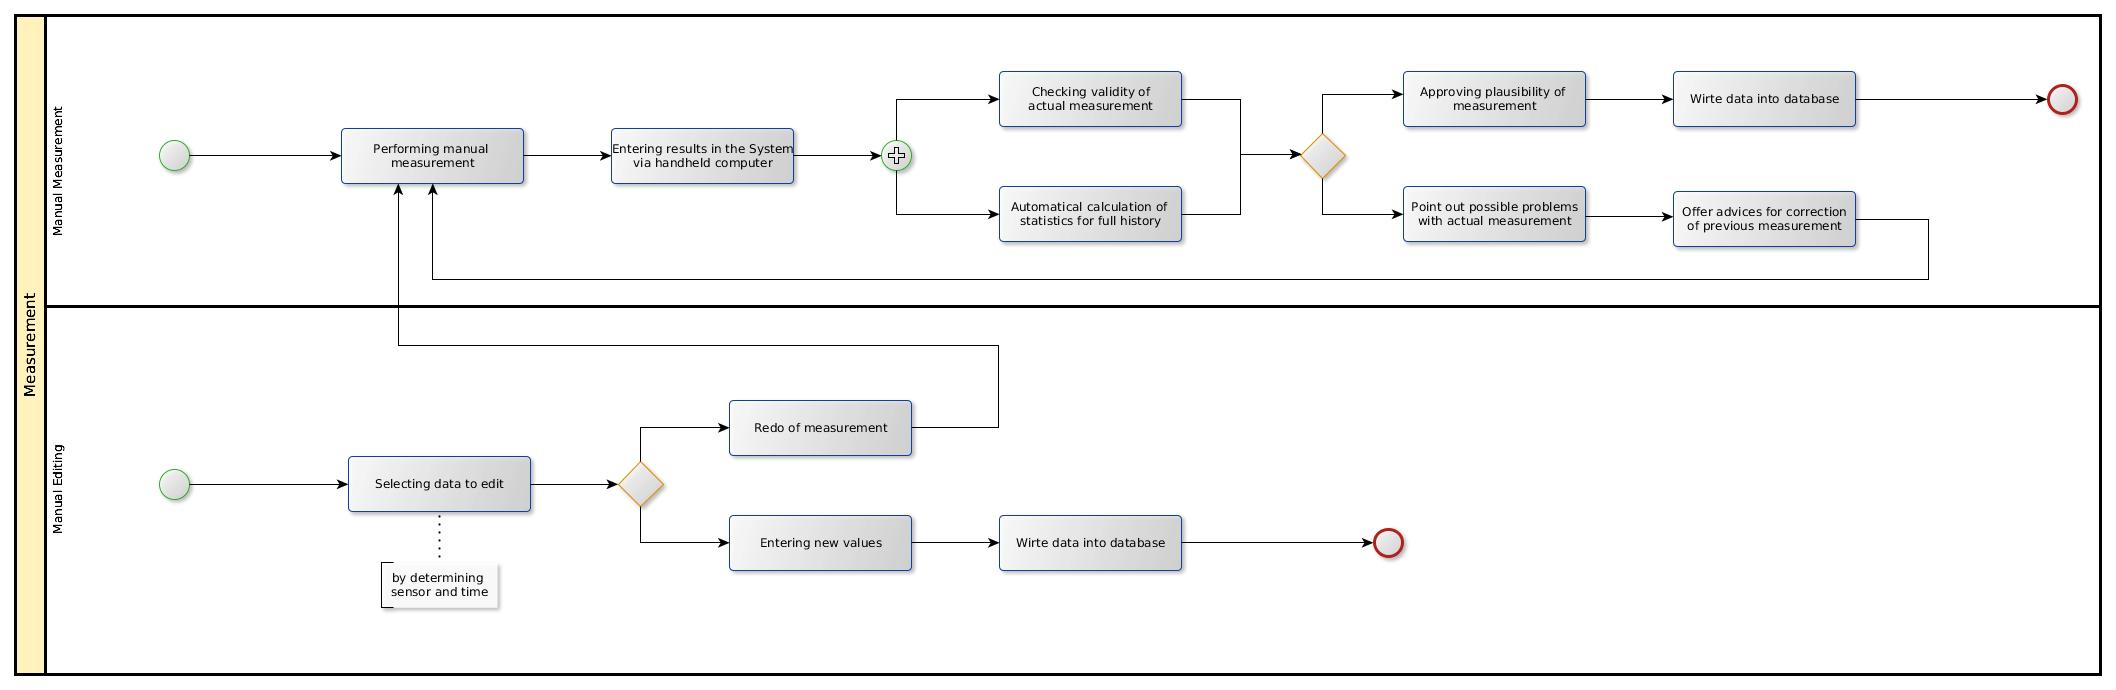
\includegraphics[scale=0.24]{graphics/bpmn_use-cases_measurement.jpg} 
	\caption{BPMN (Business Process Model and Notation) Model of the use cases describing central measuring proceedings. By F. H. Euteneuer 2013}
	 \label{fig:bpmn_use-case_measuring}
\end{figure}

\subsubsection{Analysis}

A complex part is the analysis functionalities of the system which will be described in this section. The analysis described here will be slightly different to the "ad hoc" statistics in the previous part which are leading to approved or discarded measurements. Those are checking the coherence of the performed measurements. The analysis described here are producing also easy and quick statistics, but in comparison to historical data see table \ref{table:use case description of "Analyse data"}. The user will be able to recheck if the measurements are leading to similar results, or if the measurements are possibly done with wrong parameters. 

The other analysis part is a visual analysis of the data (see table \ref{table:use case description "Visualise data"}). The system will here produce some graphics representing the measurement, the observed object and the related statistics. An optical validation of the performed measurements, and additionally to that, an optical representation of real-time data is a big advantage for the field-engineer (as described in the overall introduction).

\begin{table}[H]
\centering
\begin{tabular}{l | p{11cm}}
Name & Visualise data\\ \hline 
Usergroup & Field engineer\\ \hline 
Goal & Getting support by visualising measurements and interpretation\\ \hline 
Precondition & Existing meatadata for measurements\\ \hline 
Postcondition & meaningful and „supporting“ graphic\\
\end{tabular}
\caption{Use Cases tabular description of characteristics} 
\label{table:use case description "Visualise data"}
\end{table}

\begin{table}[H]
\centering
\begin{tabular}{l | p{11cm}}
Name & Analyse data\\ \hline 
Usergroup & Field engineer\\ \hline 
Goal & Getting information about validity of data in comparison to historical data\\ \hline 
Precondition & Amount of measurements higher then two\\ \hline 
Postcondition & information about validity of the data\\ 
\end{tabular}
\caption{Use Cases tabular description of characteristics} 
\label{table:use case description of "Analyse data"}
\end{table}

Figure \ref{fig:bpmn_use-case_analysis} is showing the two flows of the analysis part. The first line is describing the single steps of the analysis. For the analysis of data in context of historical data, the history has to be well defined. Therefore this is also part of the work-flow analysis.

The visualisation is divided into two different types of visualisations. The user can select a visualisation of the measured data. This might be represented by single geographic points. The type of visualisation is strongly depending on the type of the measurement instrument (e.g. an accelerometer is not changing its position, but it is changing the positions attributes). The second option is the visualisation of the statistics. Therefore the visualisation workflow is "calling" the function analysis in order to get the dataset specific statistics for its visualisation.

\begin{figure}[H]
	\centering
 	 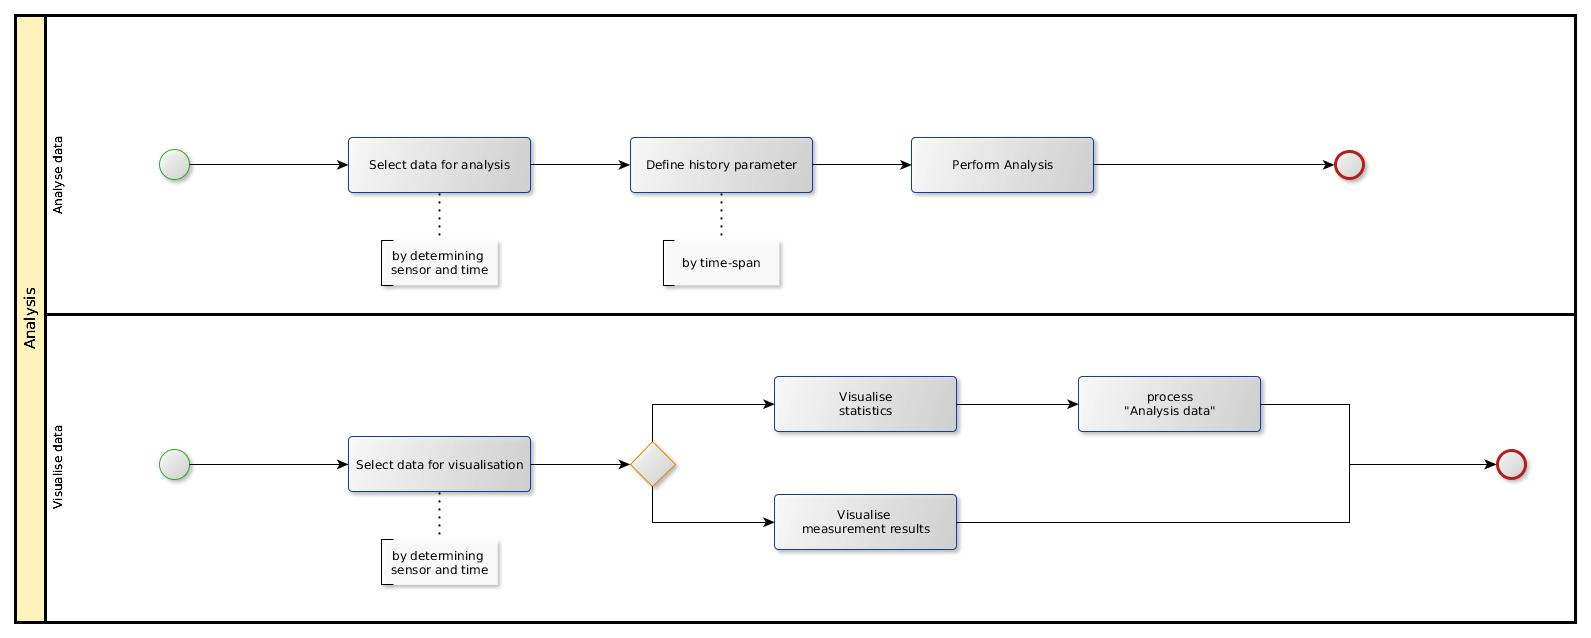
\includegraphics[scale=0.24]{graphics/bpmn_use-cases_analysis.jpg} 
	\caption{BPMN (Business Process Model and Notation) Model of the use cases describing central analysis proceedings. By F. H. Euteneuer 2013}
	 \label{fig:bpmn_use-case_analysis}
\end{figure}


\section{Product functionalities}
This part will describe the non-functional requirements of the system. This can be understood as a description of where the system will operate and how the software will operate. Non-functional requirements are requirements on a system which are not a technical functionality but a feature of the system.

The following list is describing those non-functional requirements:

\begin{description}
\item[portability] Since the system will be based on mobile devices, and those are not in any case running under windows, the software will be platform independent. Nevertheless also a web-based system is not possible, because the necessary internet connection will not be permanently available in field.
\item[performance] As described in the point before, the system will use different mobile platforms. Those do not have a hardware with a hight performance. Therefore the systems mobile part will be planed for a low performance.
\item[simplicity] The system will be used from field engineers which are working often under lots of negative influences of the environment. The system will be constructed as simply as possible to avoid unnecessary time costs for searching the right systems functionality.

\end{description}
